\usepackage{ifthen}

% Define an agenda item
%
% Arguments:
% 1: Identifier of the agenda item, should be all lower-case
% 2: Type of the agenda item: lecture or lab
% 3: English title of the agenda item
% 4: English full description of the agenda item
% 5: French title of the agenda item
% 6: French full description of the agenda item
\newcommand\defagendaitem[6]{
  \ifthenelse{\equal{\agendalanguage}{french}}{
    \expandafter\def\csname #1@#2@title\endcsname {#5}
    \expandafter\def\csname #1@#2@contents\endcsname {#6}
  }{
    \expandafter\def\csname #1@#2@title\endcsname {#3}
    \expandafter\def\csname #1@#2@contents\endcsname {#4}
  }
}

% Show/render an agenda item
%
% Arguments:
% 1: Identifier of the agenda item, as defined by \defagendaitem
% 2: Type of the agenda item: lecture or lab
\newcommand\showagendaitem[2]{%
  \ifthenelse{\boolean{hlineneeded}}{\\\hline}{\setboolean{hlineneeded}{true}}%
    \ifthenelse{\equal{\agendalanguage}{french}}{%
      \ifthenelse{\equal{#2}{lecture}}%
      {Cours &}%
      {%
        \ifthenelse{\equal{#2}{lab}}{%
          \ifthenelse{\equal{\trainingtype}{online}}{Démo &}{TP &}%
        }%
        {}%
      }%
    }{%
      \ifthenelse{\equal{#2}{lecture}}%
      {Lecture &}%
      {%
        \ifthenelse{\equal{#2}{lab}}{%
          \ifthenelse{\equal{\trainingtype}{online}}{Demo &}{Lab &}%
        }%
        {}%
      }%
    }%
    \csname #1@#2@title\endcsname &%
    \vspace{-12pt}%
    \csname #1@#2@contents\endcsname%
}%

% Define a board
%
% Arguments:
% 1: Identifier for the board, must be all lower-case
% 2: English title
% 3: English full description
% 4: French title
% 5: French full description
% 6: Board picture
\newcommand\defboard[6]{
  \ifthenelse{\equal{\agendalanguage}{french}}{
    \expandafter\def\csname #1@title\endcsname {#4}
    \expandafter\def\csname #1@contents\endcsname {#5}
  }{
    \expandafter\def\csname #1@title\endcsname {#2}
    \expandafter\def\csname #1@contents\endcsname {#3}
  }
  \expandafter\def\csname #1@image\endcsname {#6}
}

% Show/render a board
%
% Arguments:
% 1: Identifier of the board, as defined by \defboard
\newcommand\showboarditem[1]{
  \begin{tabularx}{\textwidth}{p{7cm}p{11cm}}
    \arrayrulecolor{blorange}
    \hline
    \multicolumn{1}{l}{\textbf{\textcolor{blorange}{\large \csname #1@title\endcsname}}} & \\
    \hline
    \arrayrulecolor{gray}
    \csname #1@contents\endcsname &
    \csname #1@image\endcsname \\
  \end{tabularx}
}

% Start an agenda by finding
% out if it is a morning or an
% afternoon if the training
% takes place on site
%
% Arguments:
% 1: Number of the half-day
\newcommand\showagendaday[1]{%
  \arrayrulecolor{blorange}%
  \\\hline%
  \multicolumn{3}{l}{%
    \textbf{\textcolor{blorange}{\large%
      \ifthenelse{\equal{\trainingtype}{online}}{%
        \showonlineagendaday{#1}%
      }{%
        \pgfmathparse{int(mod(#1, 2))}%
        \ifnum\pgfmathresult=1%
          \pgfmathparse{int((#1 + 1) / 2)}%
          \showonsiteagendaday{\pgfmathresult}{morning}%
        \else%
          \pgfmathparse{int(#1 / 2)}%
          \showonsiteagendaday{\pgfmathresult}{afternoon}%
        \fi%
      }%
    }}%
  } \\%
  \hline%
  \setboolean{hlineneeded}{false}%
  \arrayrulecolor{gray}%
}%

% Start an online agenda half-day
%
% Arguments:
% 1: Number of the half-day
\newcommand\showonlineagendaday[1]{%
  \ifthenelse{\equal{\agendalanguage}{french}}{%
    Demi-journée #1%
  }{%
    Half day #1%
  }%
}%

% Start an on-site agenda half-day
%
% Arguments:
% 1: Number of the day
% 2: "morning" or "afternoon"
\newcommand\showonsiteagendaday[2]{%
  \ifthenelse{\equal{\agendalanguage}{french}}{%
    \ifthenelse{\equal{#2}{morning}}{%
      Jour #1 - Matin%
    }{%
      Jour #1 - Après-midi%
    }%
  }{%
    \ifthenelse{\equal{#2}{morning}}{%
      Day #1 - Morning%
    }{%
      Day #1 - Afternoon%
    }%
  }%
}%

\defboard
{stm32mp1}
{STM32MP1 Discovery Kit}
{
  One of these Discovery Kits from STMicroelectronics: {\bf
  STM32MP157A-DK1}, {\bf STM32MP157D-DK1}, {\bf STM32MP157C-DK2} or
  {\bf STM32MP157F-DK2}
  \begin{itemize}
  \item STM32MP157, dual Cortex-A7 processor from STMicroelectronics
  \item USB powered
  \item 512 MB DDR3L RAM
  \item Gigabit Ethernet port
  \item 4 USB 2.0 host ports
  \item 1 USB-C OTG port
  \item 1 Micro SD slot
  \item On-board ST-LINK/V2-1 debugger
  \item Arduino compatible headers
  \item Audio codec, buttons, LEDs
  \item LCD touchscreen (DK2 kits only)
  \vspace{-0.7cm}
  \end{itemize}
}
{Plateforme STM32MP1}
{
  Une de ces cartes de STMicroelectronics : {\bf
  STM32MP157A-DK1}, {\bf STM32MP157D-DK1}, {\bf STM32MP157C-DK2} ou
  {\bf STM32MP157F-DK2}
  \begin{itemize}
  \item Processeur STM32MP157, double Cortex-A7, de STMicroelectronics
  \item Alimentée par USB
  \item 512 Mo DDR3L RAM
  \item Port Gigabit Ethernet port
  \item 4 ports hôte USB 2.0
  \item 1 port USB-C OTG
  \item 1 connecteur Micro SD
  \item Debugger ST-LINK/V2-1 sur la carte
  \item Connecteurs compatibles Arduino Uno v3
  \item Codec audio
  \item Divers : boutons, LEDs
  \item Écran LCD tactile (uniquement sur cartes DK2)
  \vspace{-0.7cm}
  \end{itemize}
}
{
  \begin{center}
    \includegraphics[width=5cm]{../slides/discovery-board-dk1/discovery-board-dk1.png}
  \end{center}
}

\defagendaitem
{qna}
{misc}
{Questions and Answers}
{
  \begin{itemize}
  \item Questions and answers with the audience about the course topics
  \item Extra presentations if time is left, according what most
        participants are interested in.
  \end{itemize}
}
{Questions / réponses}
{
  \begin{itemize}
  \item Questions et réponses avec les participants à propos des sujets abordés.
  \item Présentations supplémentaires s'il reste du temps, en fonction des demandes
        de la majorité des participants.
  \end{itemize}
}


\defboard
{beagleboneblack}
{BeagleBone Black}
{
  {\bf BeagleBone Black} or {\bf BeagleBone Black Wireless} board
  \begin{itemize}
  \item An ARM AM335x (single Cortex-A8) processor from Texas
    Instruments
  \item USB powered
  \item 512 MB of RAM
  \item 2 or 4 GB of on-board eMMC storage
  \item USB host and device
  \item HDMI output
  \item 2 x 46 pins headers, to access UARTs, SPI buses, I2C buses
    and more.
  \item Ethernet or WiFi
  \end{itemize}
  \vspace{-0.7cm}
}
{BeagleBone Black}
{
  Carte {\bf BeagleBone Black} ou {\bf BeagleBone Black Wireless}
  \begin{itemize}
  \item Un processeur ARM AM335x de Texas Instruments (à base de
    Cortex-A8), avec accélération 3D, etc.
  \item 512 Mo de RAM
  \item 2 ou 4 Go de stockage eMMC
  \item USB hôte et device
  \item Sortie HDMI
  \item Connecteurs à 2 x 46 broches, pour accéder aux UARTs, aux bus
    SPI, aux bus I2C, et à d'autres entrées/sorties du processeur.
  \item Ethernet ou WiFi
  \vspace{-0.7cm}
  \end{itemize}
}
{
  \begin{center}
    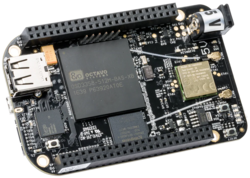
\includegraphics[width=5cm]{../slides/beagleboneblack-board/beagleboneblack_sd.png}
  \end{center}
}

\defboard
{beagleplay}
{BeaglePlay}
{
  {\bf BeaglePlay} board
  \begin{itemize}
    \item Texas Instruments AM625x (4xARM Cortex-A53 CPU)
    \item SoC with 3D acceleration, integrated MCU and many other peripherals.
    \item 2 GB of RAM
    \item 16 GB of on-board eMMC storage
    \item USB host and USB device, microSD, HDMI
    \item 2.4 and 5 GHz WiFi, Bluetooth and also Ethernet
    \item 1 MicroBus Header (SPI, I2C, UART, ...), OLDI and CSI connector.
  \vspace{-0.7cm}
  \end{itemize}
}
{BeaglePlay}
{
  Carte {\bf BeaglePlay}
  \begin{itemize}
    \item SoC Texas Instruments AM625x (CPU 4xARM Cortex-A53)
    \item SoC avec accélération 3D, MCU intégré et de nombreux autres périphériques.
    \item 2 GB de RAM
    \item 16 Go de stockage eMMC
    \item USB hôte et device, microSD, HDMI
    \item WiFi 2.4 and 5 GHz, Bluetooth et aussi Ethernet
    \item 1 Header MicroBus (SPI, I2C, UART, ...), connecteurs OLDI et CSI.
  \vspace{-0.7cm}
  \end{itemize}
}
{
  \begin{center}
    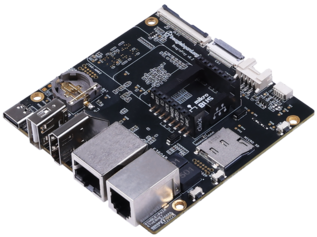
\includegraphics[width=5cm]{../slides/beagleplay-board/beagleplay_sd.png}
  \end{center}
}

\defboard
{espressobin}
{Hardware platform for practical labs}
{
  {\bf Globalscale EspressoBin} board
  \begin{itemize}
  \item Dual Cortex A53 Marvell Armada 3720 SoC
  \item Onboard switch with 2x 1Gbps interfaces
  \item Extra 1Gbps interface
  \item 1GB RAM
  \item 1x SATA interface
  \item 1x USB 3.0 interface
  \end{itemize}
}
{Plateforme matérielle pour les travaux pratiques}
{
  Carte {\bf Globalscale EspressoBin}
  \begin{itemize}
  \item SoC Marvell Armada 3720 SoC (CPU 2xARM Cortex A53)
  \item Switch Ethernet avec 2 interfaces Gigabit
  \item Interface Gigabit Ethernet additionnelle
  \item 1GB de RAM
  \item 1x interface SATA
  \item 1x interface USB 3.0
  \end{itemize}
}
{
  \begin{center}
    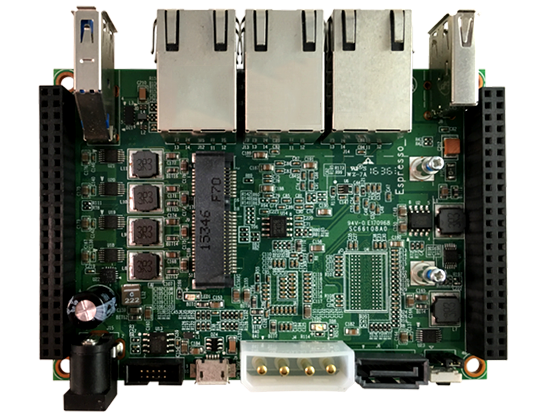
\includegraphics[width=5cm]{../slides/espressobin/espressobin.png}
  \end{center}
}


\def \training{preempt-rt}

% Title
\ifthenelse{\equal{\agendalanguage}{french}}{
  \def \trainingtitle{Formation temps-réel sous Linux avec {\em PREEMPT\_RT}}
}{
  \def \trainingtitle{Real-Time Linux with {\em PREEMPT\_RT} training}
}

% Duration
\ifthenelse{\equal{\trainingtype}{online}}{
  \def \trainingduration{3}
}{
  \def \trainingduration{2}
}

\def \trainingicon{common/flaticon-preempt-rt-training.png}

% Training objectives
\ifthenelse{\equal{\agendalanguage}{french}}{
  \def \traininggoals{
    \begin{itemize}
    \item Être capable de comprendre et de maîtriser les
      caractéristiques d'un système d'exploitation temps-réel
    \item Être capable de télécharger, compiler et utiliser le patch
      {\em PREEMPT\_RT}
    \item Être capable d'identifier et de benchmarker la plateforme
      matérielle en terme de caractéristiques temps-réel
    \item Être capable de configurer le noyau Linux pour un comportement
      déterministe
    \item Être capable de développer, de tracer et de débugger des
      applications user-space temps-réel.
    \end{itemize}
  }
}{
  \def \traininggoals{
    \begin{itemize}
    \item Be able to understand the characteristics of a real-time
      operating system
    \item Be able to download, build and use the {\em PREEMPT\_RT} patch
    \item Be able to identify and benchmark the hardware platform in
      terms of real-time characteristics
    \item Be able to configure the Linux kernel for deterministic
      behavior.
    \item Be able to develop, trace and debug real-time user-space Linux
      applications.
    \end{itemize}
  }
}

% Training prerequisites
\def \trainingprerequisites{
  \begin{itemize}
    \prerequisitecommandline
    \prerequisiteembeddedlinux
    \prerequisiteenglish
  \end{itemize}
}

% Training audience
\ifthenelse{\equal{\agendalanguage}{french}}{
  \def \trainingaudience{
    Entreprises et ingénieurs intéressés dans le développement et le
    benchmarking d'applications et de drivers temps-réel pour un
    système Linux embarqué.
  }
}{
  \def \trainingaudience{
    Companies and engineers interested in writing and benchmarking
    real-time applications and drivers on an embedded Linux system.
  }
}

% Trainers
\def \trainers {
  \href{https://bootlin.com/company/staff/maxime-chevallier/}{Maxime Chevallier}
}

% Time ratio
\def \onsitelecturetimeratio{50}
\def \onsitelabtimeratio{50}

% Agenda items

\defagendaitem
{intro}
{lecture}
{Introduction to Real-Time behaviour and determinism}
{
  \begin{itemize}
  \item Definition of a Real-Time Operating System
  \item Specificities of multi-task systems
  \item Common locking and prioritizing patterns
  \item Overview of existing Real-Time Operating Systems
  \item Approaches to bring Real-Time capabilities to Linux
  \end{itemize}
}
{Introduction au comportement temps-réel et au déterminisme}
{
  \begin{itemize}
  \item Définition d'un système d'exploitation temps-réel
  \item Spécificigés des systèmes multi-tâches
  \item Principaux patterns de verrouillage et de gestion des priorités
  \item Aperçu des systèmes temps-réel existants
  \item Approches pour apporter un comportement temps-réel à Linux
  \end{itemize}
}
\defagendaitem
{preemptrtpatch}
{lecture}
{The {\em PREEMPT\_RT} patch}
{
  \begin{itemize}
  \item History and future of the {\em PREEMPT\_RT} patch
  \item Real-Time improvements from {\em PREEMPT\_RT} in mainline Linux
  \item The internals of {\em PREEMPT\_RT}
  \item Interrupt handling: threaded interrupts, softirqs
  \item Locking primitives: mutexes and spinlocks, sleeping spinlocks
  \item Preemption models
  \end{itemize}
}
{Le patch {\em PREEMPT\_RT}}
{
  \begin{itemize}
  \item Histoire et avenir du patch {\em PREEMPT\_RT}
  \item Améliorations temps-réel provenant de {\em PREEMPT\_RT} dans le noyau Linux officiel
  \item Fonctionnement interne de {\em PREEMPT\_RT}
  \item Gestion des interruptions : interruptions threadées, softirqs
  \item Primitives de verouillage : mutexes et spinlocks, spinlocks avec sommeil
  \item Modèles de préemption
  \end{itemize}
}
\defagendaitem
{buildkernel}
{lab}
{Building a mainline Linux Kernel with the {\em PREEMPT\_RT} patch}
{
  \begin{itemize}
  \item Downloading the Linux Kernel, and applying the patch
  \item Configuring the Kernel
  \item Booting the Kernel on the target hardware
 \end{itemize}
}
{Compiler un noyau Linux avec {\em PREEMPT\_RT}}
{
  \begin{itemize}
  \item Télécharger le noyau Linux et appliquer le patch {\em PREEMPT\_RT}
  \item Configurer le noyau Linux
  \item Démarrer le kernel sur une plateforme matérielle
 \end{itemize}
}
\defagendaitem
{configuration}
{lecture}
{Hardware configuration and limitations for Real-Time}
{
  \begin{itemize}
  \item Interrupts and deep firmware
  \item Interaction with power management features: CPU frequency
    scaling and sleep states
  \item DMA
  \end{itemize}
}
{Configuration et limites du matériel pour le temps-réel}
{
  \begin{itemize}
  \item Interruptions et firmware
  \item Interaction avec les fonctionnalités de gestion d'énergie :
    gestion dynamique de la fréquence du CPU et états de sommeil
  \item DMA
  \end{itemize}
}
\defagendaitem
{tools}
{lecture}
{Tools: Benchmarking, Stressing and Analyzing}
{
  \begin{itemize}
  \item Benchmarking with {\em cyclictest}
  \item System stressing with {\em stress-ng} and {\em hackbench}
  \item The Linux Kernel tracing infrastructure
  \item Latency and scheduling analysis with {\em ftrace}, {\em
      kernelshark} or {\em LTTng}
  \end{itemize}
}
{Outils : Benchmarking, Stress et Analyse}
{
  \begin{itemize}
  \item Benchmarking avec {\em cyclictest}
  \item Stress du système avec {\em stress-ng} et {\em hackbench}
  \item L'infrastructure de {\em tracing} du noyau Linux
  \item Analyse de la latence et de l'ordonnancement avec {\em
      ftrace}, {\em kernelshark} ou {\em LTTng}
  \end{itemize}
}
\defagendaitem
{tools}
{lab}
{Tools: Benchmarking, Stressing and Analyzing}
{
  \begin{itemize}
  \item Usage of benchmarking and stress tools
  \item Common benchmarking techniques
  \item Benchmarking and configuring the hardware platform
  \end{itemize}
}
{Outils : Benchmarking, Stress et Analyse}
{
  \begin{itemize}
  \item Utilisation des outils de benchmark et de stress
  \item Techniques classiques de benchmarking
  \item Benchmarking et configuration de la plateforme matérielle
  \end{itemize}
}
\defagendaitem
{kernelinfrastructure}
{lecture}
{Kernel infrastructures and configuration}
{
  \begin{itemize}
  \item Good practices when writing Linux kernel drivers
  \item Scheduling policies and priorities: {\em SCHED\_FIFO}, {\em
      SCHED\_RR}, {\em SCHED\_DEADLINE}
  \item CPU and IRQ Affinity
  \item Memory management
  \item CPU isolation with {\em isolcpus}
  \end{itemize}
}
{Infrastructures du noyau Linux et configuration}
{
  \begin{itemize}
  \item Bonnes pratiques pour le développement de drivers noyau Linux
    pour des systèmes temps-réel
  \item Politiques d'ordonnancement et priorités : {\em SCHED\_FIFO},
    {\em SCHED\_RR}, {\em SCHED\_DEADLINE}
  \item Affinité CPU et IRQ
  \item Gestion mémoire
  \item Isolution des CPUs avec {\em isolcpus}
  \end{itemize}
}
\defagendaitem
{realtime}
{lecture}
{Real-Time Applications programming patterns}
{
  \begin{itemize}
  \item POSIX real-time API
  \item Thread management and configuration
  \item Memory management: memory allocation and memory locking, stack
  \item Locking patterns: mutexes, priority inheritance
  \item Inter-Process Communication
  \item Signaling
  \end{itemize}
}
{Patterns de développement d'applications temps-réel}
{
  \begin{itemize}
  \item API POSIX pour les applications temps-réel
  \item Gestion et configuration des threads
  \item Gestion mémoire : allocation mémoire et verouillage mémoire, gestion de la pile
  \item Patterns de verrouillage : mutexes, héritage de priorité
  \item Communication inter-processus (IPC)
  \item Signalisation
  \end{itemize}
}
\defagendaitem
{debug}
{lab}
{Debugging a demo application}
{
  \begin{itemize}
  \item Make a demo userspace application deterministic
  \item Use the tracing infrastructure to identify the cause of a latency
  \item Learn how to use the POSIX API to manage threads, locking and memory
  \item Learn how to use the CPU affinities and configure the scheduling policy
  \end{itemize}
}
{Débugger une application de démonstration}
{
  \begin{itemize}
  \item Créer une application de démonstration déterministe
  \item Utiliser l'infrastructure de {\em tracing} pour identifier la source de latence
  \item Apprendre à utiliser l'API POSIX pour gérer les threads, le verouillage, la mémoire
  \item Apprendre à utiliser l'affinité CPU et configurer la politique d'ordonnancement
  \end{itemize}
}

\def \feshowboards{
    \ifthenelse{\equal{\agendalanguage}{french}}{
      \section{Plateforme matérielle pour les travaux pratiques}
    }{
      \section{Hardware platform for practical labs}
    }

  \showboarditem{stm32mp1}
  \newpage
}

\def \onlineagenda {
  \ifthenelse{\equal{\agendalanguage}{french}}{
    \section{Programme de la formation}
  }{
    \section{Training Schedule}
  }
  \begin{tabularx}{\textwidth}{p{2cm}p{5cm}p{11cm}}
  \showagendaday{1}
  \showagendaitem{intro}{lecture}
  \showagendaitem{preemptrtpatch}{lecture}
  \showagendaitem{buildkernel}{lab}
  \showagendaitem{configuration}{lecture}
  \showagendaday{2}
  \showagendaitem{tools}{lecture}
  \showagendaitem{tools}{lab}
  \showagendaitem{kernelinfrastructure}{lecture}
  \showagendaday{3}
  \showagendaitem{realtime}{lecture}
  \showagendaitem{debug}{lab}
  \end{tabularx}
}
\def \onsiteagenda {
  \ifthenelse{\equal{\agendalanguage}{french}}{
    \section{Programme de la formation}
  }{
    \section{Training Schedule}
  }
  \begin{tabularx}{\textwidth}{p{2cm}p{5cm}p{11cm}}
  \showagendaday{1}
  \showagendaitem{intro}{lecture}
  \showagendaitem{preemptrtpatch}{lecture}
  \showagendaitem{buildkernel}{lab}
  \showagendaday{2}
  \showagendaitem{configuration}{lecture}
  \showagendaitem{tools}{lecture}
  \showagendaitem{tools}{lab}
  \showagendaday{3}
  \showagendaitem{kernelinfrastructure}{lecture}
  \showagendaitem{realtime}{lecture}
  \showagendaday{4}
  \showagendaitem{debug}{lab}
  \end{tabularx}
}
